\documentclass[12pt]{article}
\usepackage[OT4]{fontenc}
\usepackage[polish]{babel}
\usepackage[legalpaper, margin=2cm]{geometry}
\usepackage{tcolorbox}
\usepackage{float}
\usepackage{graphicx}
\usepackage{hyperref}
\usepackage{svg}
\usepackage{subcaption}

\newif\ifpokazsekcjaszesc
\pokazsekcjaszesctrue


\title{\textbf{Raport z badań z projektu zespołowego Big Data
\newline
\newline
Propozycja trasy na podstawie otwartych danych nawigacyjnych dla miasta stołecznego Warszawy}}
\author{Zespół 12: \\ Michał Zalewski \\ Jakub Próchnicki \\ Jan Machowski \\ Maciej Kurzydłowski \\ Jan Domański}
\date{Warszawa, 21 maja 2026}

\begin{document}
\maketitle
\newpage
\tableofcontents
\newpage




\section{Wstęp}

Niniejszy raport jest podsumowaniem kontynuowanych działań dążących do opracowania modelu propozycji trasy przejazdu w Warszawie,
na podstawie dostępnych jawnie danych nawigacyjnych. Główny cel tego dokumentu to przedstawienie infrastruktury stworzonej w ramach projektu, 
potoku przetwarzania danych oraz efektu działania systemu w porównaniu z istniejącymi rozwiązaniami. Opisana zostanie również wstępna analiza
wyżej wymienionego problemu oraz wnioski wyciągnięte z tej analizy.

W poprzednim dokumencie został zawarty przegląd tematyki, wstępna propozycja źródeł i narzędzi 
wykorzystanych do wykonania projektu oraz problemów i ograniczeń związanych z wybranymi danymi.

W celu przypomnienia - zaproponowana została reprezentacja miasta w postaci grafu skierowanego, 
gdzie wierzchołki są przecięciami (skrzyżowaniami) lub zakończeniami dróg, a krawędzie
są rzeczywistymi odcinkami dróg. Każda krawędź posiada odpowiedni zestaw atrybutów:
\begin{itemize}
    \item długość;
    \item typ drogi;
    \item liczba pasów;
    \item natężenie ruchu.
\end{itemize} 
Propozycja ta została wykorzystana do stworzenia wstępnego rozwiązania, opisanego w poprzednim raporcie. 
Rozwiązanie to zostało przedstawione poniżej.

Aby zachować pełnię oraz spójność dokumentu, niektóre informacje zostały powielone oraz zaktualizowane o najnowsze zmiany w projekcie
(przykładowo: opisy źródeł danych, które znajdowały się w poprzedniej wersji projektu). Dodatkowo zostaną zawarte nowe informacje dotyczące 
aspektów programu, które zostały dodane. Dzięki temu, dokument ten jest spójnym opisem całego projektu.



\section{Infrastruktura oraz potok przetwarzania danych}

\subsection{Przedstawienie infrastruktury}
Projekt został przygotowany jako środowisko skonteneryzowane w technologii \emph{Docker}. Projekt można uruchamić za pomocą komendy \verb|Docker Compose|.
Pozwala to na odtworzenie środowiska na różnych urządzeniach bez potrzeby ręcznego instalowania zależności systemowych lub bibliotek.
W kontenerze \textbf{opennavigation} znajdują się wszystkie narzędzia potrzebne do pobierania, przetwarzania i analizy danych.\\

W ramach projektu wykorzystano następujący stos technologiczny:
\begin{enumerate}
    \item \textbf{Python} - główny język implementacji;
    \item \textbf{OSMnx} i \textbf{NetworkX} - biblioteki Python'owe wykorzystywane do pracy z grafem drogowym Warszawy;
    \item \textbf{Pandas} - biblioteka wykorzystana do przetwarzania danych tabelarycznych, agregacji wyników oraz zapisu plików wynikowych;
    \item \textbf{Apache Kafka} - system wymiany danych umożliwiający przesyłanie danych w różnych etapach potoku przetwarzania danych;
    \item \textbf{Apache Spark} - rozwiązanie wykorzystywane do przetwarzania danych stumieniowych oraz transformację surowych danych w dane gotowe do analizy.
\end{enumerate}

\noindent W projekcie nie wykorzystano czystego Hadoopa, co jest zgodne z przyjętym zakresem projektu - technologia ta była traktowana
jako opcjonalne narzędzie. Zamiast tego, dane są przetwarzane lokalnie a wyniki są zapisywane w strukturze katalogów projektu.\\

\noindent Struktura danych w projekcie podzielona jest na trzy katalogi:
\begin{itemize}
    \item \textbf{data/raw} - katalog przechowujący dane surowe, m.in. raporty XLSX/PDF zaczerpnięte ze źródeł zewnętrznych;
    \item \textbf{data/processed} - katalog przechowujący dane oczyszczone oraz zagregowane, wykorzystywane do zadania analizy tras;
    \item \textbf{data/results} - katalog przechowujący wyniki analiz - m.in. porównanie tras.
\end{itemize}

\noindent \\W obecnej wersji projektu, możliwe jest uruchomienie pełnej analizy trasy w następujących krokach:
\begin{enumerate}
    \item Pobranie danych źródłowych (raporty XLSX/PDF z zewnętrznych źródeł);
    \item Przetworzenie danych (czyszczenie, transformacja, agregacja);
    \item Wyznaczenie trasy na podstawie przetworzonych danych;
    \item Porównanie różnych wariantów trasy według odpowiednich funkcji kosztu.
\end{enumerate}

\subsection{Potok danych}

\noindent Potok danych został przygotowany w sposób, który umożliwia łączenie różnych źródła danych w jeden, spójny model kosztu przejazdu.\\

\noindent Podstawą analizy jest graf drogowy Warszawy, stworzony na podstawie danych pobranych z \textbf{OpenStreetMap} za pomocą biblioteki \textbf{OSMnx}. 
Pierwotny, pobrany graf jest wzbogacany o następujące dane:
\begin{itemize}
    \item \textbf{ZDM} - dane dotyczące natężenia ruchu oraz średnich prędkości pojazdów. Dane te są punktowe, więc są wykorzystywane do korekty
                            kosztu przejazdu tylko dla tych krawędzi, dla których są dostępne. W ramach poprawy modelu, można wykorzystać alternatywne
                            źródło strumieniowych danych \textbf{TomTom} opisane poniżej;
    \item \textbf{Dane pogodowe} - dane dotyczące warunków pogodowych, które wpływają na czas przejazdu - deszcz, mgła etc.
\end{itemize}

\noindent \\\textbf{Potok} obejmuje następujące etapy:
\begin{itemize}
    \item Pobór danych;
    \item Czyszczenie i transformację danych;
    \item Agregację danych do postaci użytecznej w analizie tras;
    \item Zapis wyników pośrednich i końcowych.
\end{itemize}

\noindent \\Szczegółowy opis poszczególnych etapów potoku przedstawiono w kolejnych podpunktach.

\subsubsection{Źródła danych}
Źródła danych obejmują zarówno statyczny opis sieci drogowej, jak i dane zmienne w czasie.
W projekcie wykorzystano następujące źródła:
\begin{itemize}
    \item \textbf{OpenStreetMap / Overpass API} - źródło zawierające geometrię sieci drogowej Warszawy oraz atrybuty
    odcinków (np. \textit{highway}, \textit{maxspeed}, \textit{lanes}, \textit{oneway}). Te dane stanowią
    podstawę do budowy grafu ulic oraz wyznaczenia bazowych czasów przejazdu.
    Przykład zapytania Overpass API używanego w projekcie (wybór dróg głównych dla Warszawy):
\begin{tcolorbox}
\begin{verbatim}
[out:json][timeout:120];
area["name"="Warszawa"]->.a;
(
    way["highway"~"^(primary|secondary|tertiary)$"](area.a);
);
(._;>;);
out body;
\end{verbatim}
\end{tcolorbox}

Przykładowy fragment odpowiedzi (rzeczywisty wynik, ograniczony do pojedynczego odcinka dla czytelności):
\begin{tcolorbox}
\begin{verbatim}
{
    "elements": [
        {
            "type": "way",
            "id": 4307329,
            "nodes": [
                2448759046,
                7093785352,
                2452307268,
                1439574696
            ],
            "tags": {
                "cycleway:both": "no",
                "highway": "tertiary",
                "junction": "roundabout",
                "lane_markings": "no",
                "lit": "yes",
                "maxspeed": "50",
                "name": "Rondo Feliksa Stamma",
                "name:etymology:wikidata": "Q5441838",
                "sidewalk:left": "no",
                "sidewalk:right": "separate",
                "source:maxspeed": "PL:urban",
                "surface": "asphalt",
                "wikidata": "Q113528575"
            }
        }
    ]
}
\end{verbatim}
\end{tcolorbox}

    \item \textbf{ZDM Warszawa (APR)} - źródło zawierające punktowe pomiary natężenia ruchu na wybranych odcinkach.
    Dane są pobierane z panelu \textit{Analiza ruchu na drogach online}
   {\sloppy (\url{https://zdm.waw.pl/dzialania/badania-i-analizy/analiza-ruchu-na-drogach/analiza-ruchu-na-drogach-online/})\fussy}
    w postaci raportu XLSX.
    Pobieranie jest zautomatyzowane skryptem \verb|zdm_online_traffic_loader.py|,
    który steruje interfejsem WWW (Playwright) i zapisuje raport do pliku.
    
    Tabela \ref{tab:zdm-apr-format} przedstawia uproszczony format rekordu APR, który trafia do potoku danych
    po wczytaniu raportu XLSX.

    \begin{table}[H]
        \centering
        \caption{Format danych ZDM APR (po wczytaniu do potoku)}
        \label{tab:zdm-apr-format}
        \begin{tabular}{|l|p{10cm}|}
            \hline
            \textbf{Pole} & \textbf{Opis} \\ \hline
            source & Identyfikator źródła (np. \textit{zdm\_apr\_real}). \\ \hline
            station\_id & Id punktu pomiarowego ZDM. \\ \hline
            station\_name & Nazwa punktu pomiarowego (np. ulica/sekcja). \\ \hline
            road\_name & Nazwa ulicy. \\ \hline
            section & Opis odcinka (np. między skrzyżowaniami). \\ \hline
            direction & Kierunek pomiaru. \\ \hline
            lat, lon & Współrzędne geograficzne punktu. \\ \hline
            measurement\_time & Czas pomiaru w formacie \textit{YYYY-MM-DD HH:00:00}. \\ \hline
            period\_minutes & Okno czasowe pomiaru (zwykle 60). \\ \hline
            vehicle\_count & Liczba pojazdów w danym oknie. \\ \hline
            avg\_speed\_kmh & Brak w APR (pole puste). \\ \hline
            \_metadata & Metadane techniczne: czas wczytania, plik źródłowy, arkusz. \\ \hline
        \end{tabular}
    \end{table}

    \item \textbf{Raporty prędkości ZDM (PDF)} - źródło zawierające cykliczne raporty z uśrednionymi prędkościami,
    publikowane na pulpicie ZDM
    (\url{https://zdm-warszawa.maps.arcgis.com/apps/dashboards/20bfffc9bae544b5a1cdfaad7be38c40}).
    Pobieranie plików jest zautomatyzowane skryptem \verb|zdm_speed_report_downloader.py|.
    Następnie skrypt \verb|zdm_speed_pdf_parser.py| przetwarza pliki PDF do formatu CSV
    (\verb|zdm_speed_measurements.csv|).

    Tabela \ref{tab:zdm-speed-format} pokazuje uproszczony format rekordu z raportów prędkości.

    \begin{table}[H]
        \centering
        \caption{Format danych ZDM -- raporty prędkości (po parsowaniu PDF)}
        \label{tab:zdm-speed-format}
        \begin{tabular}{|l|p{10cm}|}
            \hline
            \textbf{Pole} & \textbf{Opis} \\ \hline
            source & Identyfikator źródła (np. \textit{zdm\_speed\_pdf}). \\ \hline
            source\_file & Nazwa pliku PDF, z którego pochodzi rekord. \\ \hline
            station\_id & Id punktu pomiarowego ZDM. \\ \hline
            station\_name & Nazwa punktu (np. ulica/sekcja). \\ \hline
            road\_name & Nazwa ulicy. \\ \hline
            direction & Kierunek pomiaru. \\ \hline
            lat, lon & Współrzędne geograficzne punktu. \\ \hline
            measurement\_date & Data raportu (YYYY-MM-DD). \\ \hline
            measurement\_time & Znaczniki czasu (domyślnie 00:00:00). \\ \hline
            period\_minutes & Okres uśrednienia (1440 minut). \\ \hline
            day\_of\_week & Dzień tygodnia z raportu. \\ \hline
            vehicle\_count & Liczba pojazdów (jeśli dostępna). \\ \hline
            avg\_speed\_kmh & Średnia prędkość dla kierunku/dnia. \\ \hline
            avg\_speed\_day\_kmh & Średnia prędkość w dzień. \\ \hline
            avg\_speed\_night\_kmh & Średnia prędkość w nocy. \\ \hline
            avg\_speed\_light\_kmh & Prędkość dla pojazdów lekkich. \\ \hline
            avg\_speed\_heavy\_kmh & Prędkość dla pojazdów ciężkich. \\ \hline
            vmax\_kmh, v85\_kmh & Prędkości Vmax i V85 (jeśli dostępne). \\ \hline
            vdop\_raw & Dopuszczalna prędkość (surowy zapis z PDF). \\ \hline
        \end{tabular}
    \end{table}
        \item \textbf{Open-Meteo} - źródło danych pogodowych w podziale godzinowym - opady, wiatr, widoczność, temperatura.
        Pobieranie z API realizuje skrypt
        \verb|weather_loader.py|, który zapisuje pełny plik JSON do tematu Kafki
        (temat \textit{warszawa-raw-weather}). Dane te stanowią kontekst do dodatkowej korekty kosztu.

        Przykład zapytania API (parametry używane w projekcie):
        \begin{tcolorbox}
        \begin{verbatim}
    https://api.open-meteo.com/v1/forecast?
    latitude=52.2297&
    longitude=21.0122&
    hourly=temperature_2m,precipitation,rain,snowfall,wind_speed_10m,
    visibility,weather_code&
    forecast_days=1&
    timezone=Europe/Warsaw
        \end{verbatim}
        \end{tcolorbox}

        Przykładowy fragment odpowiedzi (rzeczywisty wynik, skrócony do kilku godzin):
        \begin{tcolorbox}
        \begin{verbatim}
{
    "latitude": 52.23009,
    "longitude": 21.017075,
    "timezone": "Europe/Warsaw",
    "hourly": {
        "time": [
            "2026-05-22T00:00",
            "2026-05-22T01:00",
            "2026-05-22T02:00"
        ],
        "temperature_2m": [16.9, 15.9, 14.9],
        "precipitation": [0.0, 0.0, 0.0],
        "wind_speed_10m": [11.2, 8.6, 6.1],
        "weather_code": [3, 0, 3]
    }
}
        \end{verbatim}
        \end{tcolorbox}
        \item \textbf{TomTom} - źródło danych strumieniowych, z którego pozyskiwane są informacje dotyczące szacowanych, aktualnych 
        prędkości oraz czasów przejazdu na drogach najbliższych do wybranych, wysłanych przez użytkownika API współrzędnych - wszystkie te dane są, 
        oczywiście, obarczone współczynnikiem pewności \emph{confidence}.

        Wykorzystanie tych danych realizuje skrypt \verb|tomtom_traffic_loader.py| zapisujący dane w Kafce pod tematem \emph{warszawa-raw-traffic}.
        Dzięki tym danym, które po transformacji za pomocą \verb|tomtom_edge_mapping| są transformowane do formatu obsługiwanego przez instniejący plik  
        \verb|zdm_traffic_aggregation.py|, stanowią dodatkową podstawę do analizy korków na drogach Warszawy. \emph{Dane te są przekształcone i wykorzystywane
        w analogiczny sposób co dane ZDM, więc w sekcji \ref{sssec:czyszczenie} transformacje tych danych nie będą dodatkowo opisywane.}
        W ramach zyskania dostęp do danych TomTom potrzebny jest klucz API. Można go zdobyć bezkosztownie na stronie \emph{my.tomtom.com}. Po uzyskaniu
        należy owy klucz wstawić do pliku \verb|.env|.

        W projekcie, w celu pobrania danych wykorzystywane jest zapytanie GET. Przykład wykorzystania API TomTom oraz uzyskanych od niego 
        informacji znajduje się poniżej:
        \begin{tcolorbox}
            \begin{verbatim}
{
    https://api.tomtom.com/traffic/services/4/flowSegmentData/absolute/
    10/json,
    params={
        "key": TOMTOM_API_KEY,
        "point": f"{52.218662},{21.017080}",
        "unit": "KMPH",
        "style": "relative",
    },
    timeout=30,
}

...

{
  "flowSegmentData": {
    "-xmlns": "http://lbs.tomtom.com/services",
    "-version": "traffic-service 2.0.004",
    "frc": "FRC2",
    "currentSpeed": 34,
    "freeFlowSpeed": 50,
    "currentTravelTime": 43,
    "freeFlowTravelTime": 30,
    "confidence": 0.71,
    "roadClosure": true,
    "coordinates": {
      "coordinate": [
        {
          "latitude": 52.218662,
          "longitude": 21.017082
        }
      ]
    }
  }
}
            \end{verbatim}
        \end{tcolorbox}


\end{itemize}

\begin{figure}[H]
    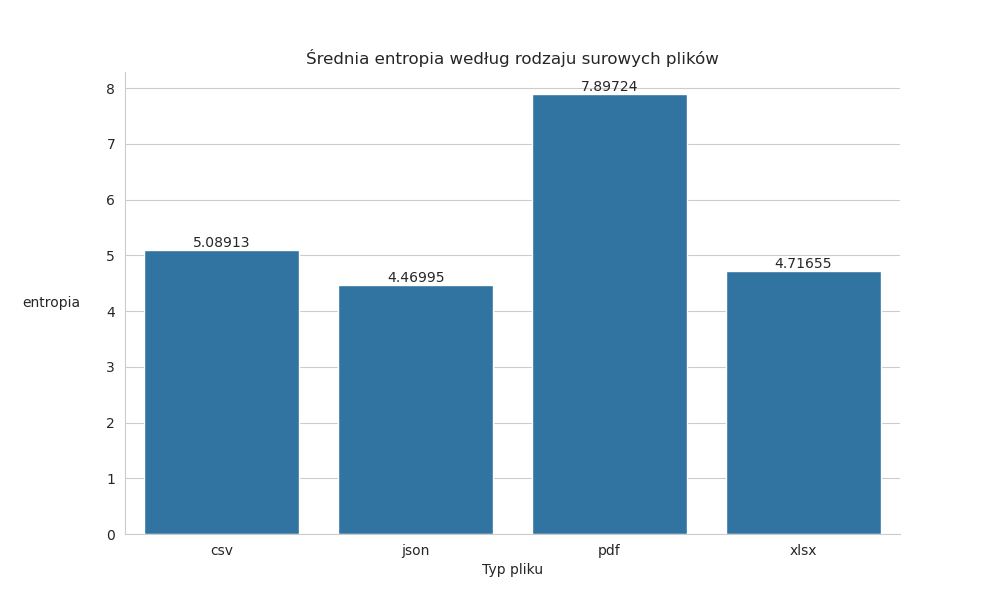
\includegraphics[width=0.9\textwidth]{png/avg_entropy_by_type.png}
    \caption{Średnia entropia, rozumiana w sensie teorii informacji, dla poszczególnych typów plików źródłowych (nieprzetworzonych)}
\end{figure}

\subsubsection{Struktura surowych danych - wykresy}

\begin{figure}[H]
    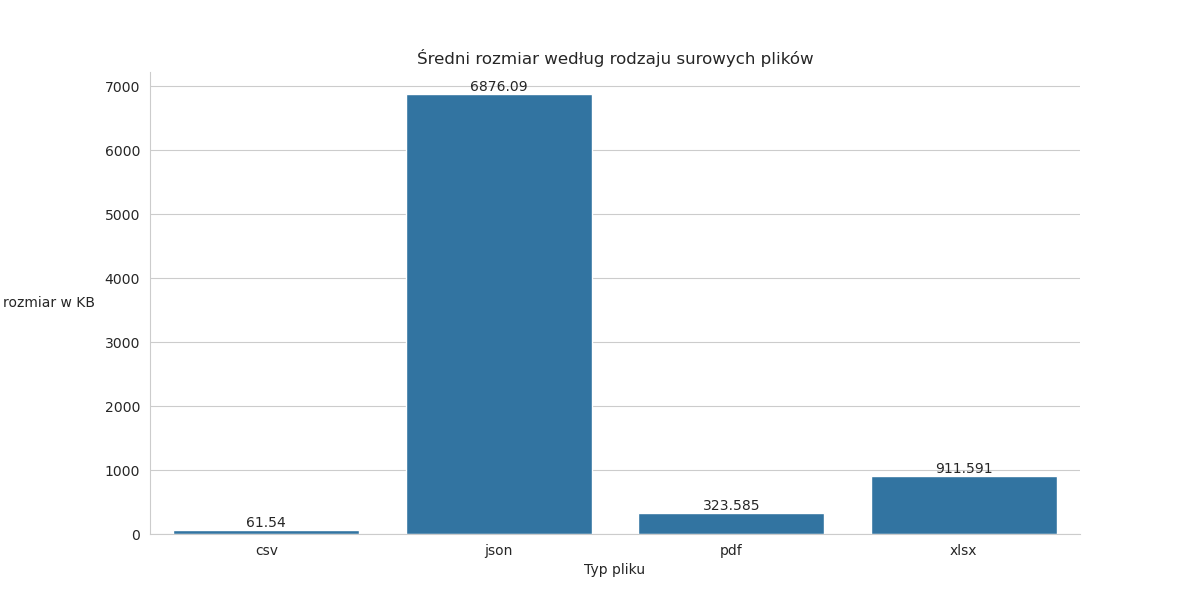
\includegraphics[width=0.9\textwidth]{png/avg_size_by_type.png}
    \caption{Średni rozmiar pliku źródłowego według typu pliku źródłowego (nieprzetworzonego)}
\end{figure}

Pliki typu pdf są najmniej ustrukturyzowanym źródłem danych w naszym projekcie, co potwierdza
wysoka entropia zawartości tych plików. Największy udział w danych źródłowych pod względem rozmiaru
mają pliki w formacie JSON, które jednocześnie charakteryzuje najmniejsza entropia, co może
oznaczać najwyższy poziom ustrukturyzowania spośród wszystkich wykorzystywanych typów plików.
\subsubsection{Pobór danych - Kafka}
Pobór danych realizowany jest przez skrypty wczytujące, które zapisują dane wejściowe jako
wiadomości JSON w tematach Apache Kafka. Poniżej znajduje się zestawienie przyjmowanych przez Kafkę danych z podziałem 
na poszczególne tematy oraz dalszy kierunek przekazywania danych:
\begin{itemize}
    \item \textbf{warszawa-raw-streets} -- 
    \begin{itemize} 
        \item Źródło: Overpass API;
        \item Producent: \path{overpass_raw_street_loader.py};
        \item Konsument: \path{overpass_transformations.py}; 
        \item Zapis do katalogu: \path{/app/data/processed/osm_ways} 
        \item Publikacja do tematu: \textit{warszawa-processed-edges}.
    \end{itemize}
    \item \textbf{warszawa-raw-traffic}
    \begin{itemize} 
        \item Źródło: ZDM / TomTom;
        \item Producent: \path{zdm_traffic_loader.py} lub \path{traffic_loader.py};
        \item Konsument: \path{traffic_transformations.py}; 
        \item Zapis do katalogu: \path{/app/data/processed/traffic_measurements};
        \item Późniejsza agregacja: \path{zdm_traffic_aggregation.py}, \path{/app/data/processed/zdm_traffic_by_road.csv}.
    \end{itemize} 
    \item \textbf{warszawa-raw-weather}
    \begin{itemize} 
        \item Źródło: Open-Meteo;
        \item Producent: \path{weather_loader.py};
        \item Konsument: \path{weather_transformations.py}; 
        \item Zapis do katalogu: \path{/app/data/processed/weather_observations}.
    \end{itemize} 
    \item \textbf{warszawa-processed-edges} -- ujednolicone krawędzie grafu po transformacji OSM;
    temat wyjściowy z \path{overpass_transformations.py}, możliwy do dalszego
    wykorzystania analitycznego.
\end{itemize}

W obecnej wersji zasilanie odbywa się wsadowo (mikro-batch), jednak potok działa w trybie
strumieniowym po stronie Apache Spark. Kafka pełni rolę bufora i kolejki zdarzeń,
co zwiększa powtarzalność obliczeń i pozwala na odtwarzanie danych od wybranego offsetu.

\subsubsection{Czyszczenie i transformacja danych - Apache Spark, OSMnx}
\label{sssec:czyszczenie}
W ramach tego etapu, dane debrane w zasobach Kafki są przekształcane do postaci, która zostanie wykorzystana w późniejszym etapie - analizie tras.

Dane \textbf{ZDM APR} są pobirane do Apache Kafka w surowej postaci, a następnie przetwarzane z pomocą Apache Spark. Skonfigurowane rozwiązanie Spark
odczytuje komunikaty z tematu \textbf{warszawa-raw-traffic}, które są w formacie JSON, po czym analizuje oraz przekształca je do postaci tabelarycznej.
W ramach tego procesu, program ujednolica nazwy kolumn, konwertuje czas pomiaru do formatu daty i czasu oraz przelicza liczbę pojazdów w postać 
natężenia ruchu - $natezenie = \frac{l. pojazdow}{h}$.

Na tym etapie wyznaczany jest również współczynnik \textbf{traffic\_factor}, który jest później wykorzystywany jako \textbf{kara kosztu przejazdu}
dla ulic, które mają dostępne pomiary natężenia ruchu.\\

W trakcie transformacji dochodzi do agregacji danych \textbf{ZDM APR} po ulicach - z wielu rekordów godzinowych wybierane są maksymalne/średnie wartości 
\textbf{traffic\_factor}, liczby pomiarów oraz zakresy dat. Wynikiem tych operacji jest plik \textbf{zdm\_traffic\_by\_road.csv}, pozwalający na 
uruchomienie analizy tras bez ponownej potrzeby przetwarzania dużych danych wejściowych.\\

Proces czyszczenia i transformacji dla danych o dozwolonych prędkościach z \emph{ZDM} (w formie PDF) jest bardziej złożony.
Dane są przetwarzane osobnym analizatorem składniowym. Pobierane są zawartości plików PDF a następnie wydobywane są z nich kluczowe informacje, takie jak:
\begin{itemize}
    \item Identyfikator punktu pomiarowego;
    \item Nazwa ulicy;
    \item Lokalizacja (współrzędne geograficzne);
    \item Data pomiaru;
    \item Średnia prędkość \textbf{avg\_speed\_kmh}.
    
\end{itemize}

W przypadku, w którym dla konkretnej ulicy istnieje wiele pomiarów średniej prędkości w różnych odstępach czasowych, na tych danych również wykonywana
jest agregacja. Jeżeli informacja dotycząca liczby pojazdów jest dostępna, wyznaczana jest średnia ważona, gdzie waga jest liczbą pojazdów. W przeciwnym
razie, wyznaczana jest średnia arytmetyczna.

\newpage

Wykorzystując bibliotekę \textbf{OSMnx}, system tworzy strukturę sieci drogowej Warszawy. Dla danego obszaru miasta pobierany jest graf drogowy o typie
\emph{network\_type = 'drive'}\footnote{Typy grafów są jednoznaczne z przeznaczeniem danej drogi, tj. ulica, trasa rowerowa, chodnik etc. \\ Listę dostępnych 
typów można znaleźć w dokumentacji OSMnx: \url{https://osmnx.readthedocs.io/en/stable/user-reference.html\#osmnx.graph.graph_from_address}},
który odpowiada ulicom przeznaczonym dla pojazdów. Dla tych ulic, bazowe prędkości/czasu przejazdu dla krawędzi są wyznaczane automatycznie, 
po czym są wzbogacane o następujące atrybuty:
\begin{itemize}
    \item \textbf{traffic\_factor} - korekta kosztu przejazdu na podstawie ZDM APR - danych o natężeniu ruchu;
    \item \textbf{speed\_factor} - korekta na podstawie prędkości ruchu z raportów ZDM;
    \item \textbf{weather\_factor} - korekta na podstawie danych o pogodzie;
    \item \textbf{traffic\_speed\_factor} - ostateczna korekta wynikająca z danych ruchu i prędkości - jest ona wyznaczana jako maksimum z wartości \textbf{traffic\_factor} i \textbf{speed\_factor};
    \item \textbf{cost\_time\_s} - końcowa waga krawędzi w grafie, będąca wartością czasu w sekundach, uwzględniająca bazowy czas przejazdu i dostępne korekty.
\end{itemize}

Dodatkową, istotną operacją wykonywaną podczas transformacji danych jest normalizacja nazwy ulic. 
Dane ZDM są dopasywane do poszczególnych krawędzi grafu względem nazwy ulic, a OpenStreetMap oraz ZDM często posiadają różne 
formy zapisu konkretnych nazw ulic, przykładowo: Al. lub Aleje, Ul. lub Ulica, \dots Transformator danych stosuje uproszczone, ujednolicone 
nazwy ulic - w celu osiągnięcia tego efektu usuwane są wybrane skróty.

Na etapie transformacji normalizowane są też nazwy ulic, bowiem ZDM oraz OpenStreetMap mogą mieć różne formy zapisu nazw konkretnych ulic, np. Al. i Aleje. Potok stosuje uproszczone ujednolicanie nazw i usuwanie wybranych skrótów. Jest to istotne, ponieważ dane ZDM są głównie dopasowywane do krawędzi po nazwach ulic, co na późniejszym etapie zostanie zastąpione dopasowniem przestrzennym.\\


\subsubsection{Zapis danych}

Po oczyszczeniu, przekształceniu i wzbogaceniu danych o dodatkowe atrybuty odbywa się ich zapis do poszczególnych katalogów w projekcie.
W tej kwestii zastosowano następujący podział:
\begin{itemize}
    \item Dane surowe, takie jak raporty XLSX/PDF, są zapisywane w katalogu \textbf{data/raw};
    \item Dane przetworzone, takie jak pomiary natężenia ruchu czy dane pogodowe, są zapisywane w katalogu \textbf{data/processed}. Format zapisu dla danych tabelarycznych to \emph{Parquet};
    \item Wyniki analiz są zapisywane w katalogu \textbf{data/results}. 
\end{itemize}

\subsubsection{Diagram potoku danych}
Potok danych można całokształtnie przedstawić na następującym diagramie:

\begin{figure}[H]
    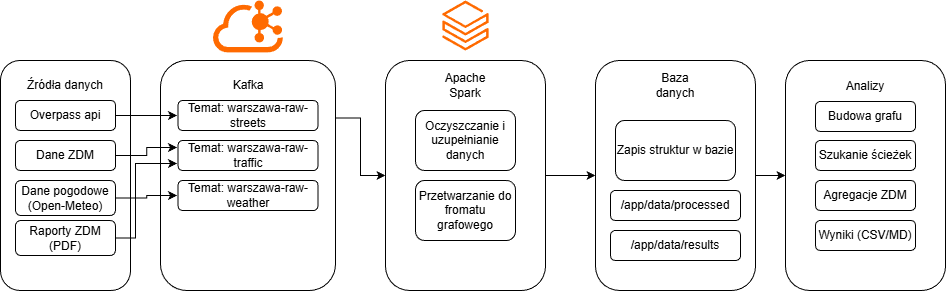
\includegraphics[width=\textwidth]{png/OpenNavigationArchitecture.png}
    \caption{Diagram potoku danych.}
\end{figure}

\newpage
\section{Instalacja, konfiguracja oraz wykonanie projektu}

\subsection{Instalacja i zbudowanie projektu}

Aktualną wersję rozwiązania można znaleźć w otwartym repozytorium na GitHub, pod linkem \url{https://github.com/JacobPW23/OpenNavigation}.

Aby zapewnić uniwersalność rozwiązania i prostotę obsługi i udostępniania postanowiono skonteneryzować projekt 
za pomocą technologi Docker. W celu wykorzystania OpenNavigation należy sklonować repozytorium, zbudować obraz oraz 
uruchomić kontener na podstawie zbudowanego obrazu:

\begin{tcolorbox}
\begin{verbatim}
git clone https://github.com/JacobPW23/OpenNavigation
cd OpenNavigation
docker compose build
docker compose up -d
\end{verbatim}
\end{tcolorbox}

Należy zwrócić uwagę, iż z powodu instalowania narzędzi Apache, zbudowanie obrazu Docker'a może chwilę zająć.

\subsection{Pobór danych (ingestion)}
Pobieranie danych jest zautomatyzowane za pomocą skryptów Pythona, które można uruchomić w kontenerze Docker.
Poniżej przedstawiono komendy do pobrania danych z poszczególnych źródeł:

\par\medskip
\textbf{Dane APR ZDM}
\begin{tcolorbox}
\begin{verbatim}

docker compose exec opennavigation python \
src/ingestion/zdm_online_traffic_loader.py

docker compose exec opennavigation python \
src/ingestion/zdm_traffic_loader.py

docker compose exec opennavigation spark-submit \
--packages \
org.apache.spark:spark-sql-kafka-0-10_2.12:3.5.1 \
src/processing/traffic_transformations.py

docker compose exec opennavigation python \
src/analysis/zdm_traffic_aggregation.py
\end{verbatim}
\end{tcolorbox}
Wyniki: \path{data/processed/zdm_traffic_by_road.csv}.

\par\medskip
\textbf{Raporty prędkości ZDM (PDF)}
\begin{tcolorbox}
\begin{verbatim}
docker compose exec opennavigation python \
src/ingestion/zdm_speed_report_downloader.py

docker compose exec opennavigation python \
src/ingestion/zdm_speed_pdf_parser.py

docker compose exec opennavigation python \
src/analysis/zdm_speed_aggregation.py
\end{verbatim}
\end{tcolorbox}
Wyniki: \path{data/processed/zdm_speed_by_road.csv}.

\par\medskip
\newpage
\textbf{OSM / Overpass}
\begin{tcolorbox}
\begin{verbatim}
docker compose exec opennavigation python \
src/ingestion/overpass_raw_street_loader.py

docker compose exec opennavigation spark-submit \
--packages \
org.apache.spark:spark-sql-kafka-0-10_2.12:3.5.1 \
src/processing/overpass_transformations.py
\end{verbatim}
\end{tcolorbox}
Wyniki: temat \textit{warszawa-processed-edges}.

\par\medskip
\textbf{Pogoda (Open-Meteo)}
\begin{tcolorbox}
\begin{verbatim}
docker compose exec opennavigation python \
src/ingestion/weather_loader.py

docker compose exec opennavigation spark-submit \
--packages \
org.apache.spark:spark-sql-kafka-0-10_2.12:3.5.1 \
src/processing/weather_transformations.py
\end{verbatim}
\end{tcolorbox}
Wyniki: \textit{warszawa-raw-weather}.

\subsection{Konfiguracja skryptów analizy}

% do sprawdzenia poprawności
Po udanym postawieniu kontenera, i sprawdzeniu jego działania za pomocą \verb|docker compose ps|, dane 
mogą zostać pobrane według potoku danych.

Skrypty wykonujące analizę optymalnej trasy na podstawie danych znajdują się pod następującymi ścieżkami:
\begin{itemize}
\item \verb|/app/src/analysis/route_initial_analysis.py|
\item \verb|/app/src/analysis/osm_initial_analysis.py|
\end{itemize}

\Huge

TODO - opis pozostałych skryptów

\normalsize

W tym raporcie opisane zostanie wykorzytanie pierwszego skryptu. Pozostałe zostaną opisane w ramach raportu końcowego.

Kluczowym punktem dla analizy jest zdefiniowana w tym pliku stała \textbf{ROUTES}, w której określone są punkty 
początkowe i końcowe, dla których ma zostać znaleziona optymalna trasa.
Poniżej zamieszczono przykładową konfigurację zmiennej, domyślnie znajdującą się w skrypcie w języku Python:

\begin{tcolorbox}
    \begin{verbatim}
ROUTES = [
    {
        "route_name": "Mokotowska -> Dobra",
        "origin": (52.218662, 21.017080),
        "destination": (52.244974, 21.020670),
    },
]
    \end{verbatim}
\end{tcolorbox} 
gdzie współrzędzne \textit{origin} oraz \textit{destination} są podawane jako \textit{(latitude, longitude)}.

Aby uruchomić analizę tras, należy wykonać plik analizy tras po wprowadzeniu swojej konfigurazji. Komenda:
\begin{tcolorbox}
    \begin{verbatim}
docker compose exec opennavigation python \
src/analysis/route_initial_analysis.py
    \end{verbatim}
\end{tcolorbox} 


\subsection{Dane wyjściowe}
Wyniki wykonania skryptu znajdą się w katalogu \verb|/app/data/results/route_initial_analysis/|. Dla analizy danych 
istotne są 3 pliki wynikowe:
\begin{enumerate}
    \item summary.md - podsumowanie wyniku analizy skryptu;
    \item routes\_comparison.csv - plik csv podsumowujący najważniejsze aspekty determinujące proponowane trasy:
    distance\_km, base\_time\_min, adjusted\_time\_min, traffic\_impacted\_edges, \\
    speed\_impacted\_edges, zdm\_apr\_edges, zdm\_speed\_edges, osmnx\_only\_edges; 
    \item route\_edges.csv - szczegóły krawędzi optymalnej trasy znalezionej przez algorytm, takie jak 
            traffic\_factor, speed\_factor, traffic\_speed\_factor, measured\_avg\_speed\_kmh, cost\_source.
\end{enumerate}



\section{Wstępna analiza problemu}

\subsection{Cel i metodyka}
Celem rozdziału jest weryfikacja, czy algorytm znajduje sensowną trasę oraz czy czas przejazdu
w minutach jest liczony spójnie. Dodatkowo wyniki porównano z czasami i dystansami z Google Maps
dla aktualnego obciążenia ruchu (19:00--19:30), aby ocenić zgodność kierunkową.
Analiza opiera się na wynikach generowanych przez \verb|route_initial_analysis.py| i zapisanych w
\path{data/results/route_initial_analysis}.

Przyjęta metodyka:
\begin{enumerate}
    \item Wybrano trzy pary punktów start--cel (\textit{ROUTES}).
    \item Dla każdej pary wyznaczono trzy warianty: najkrótszy dystansowo, najszybszy bazowo
    (na podstawie \textit{travel\_time} z OSMnx) oraz wariant skorygowany
    (\textit{cost\_time\_s} z uwzględnieniem danych ZDM i pogody).
    \item Dla każdej trasy zsumowano długość oraz czasy przejazdu, uzyskując
    \textit{distance\_km}, \textit{base\_time\_min} i \textit{adjusted\_time\_min}.
    \item Wygenerowane trasy przepisano do Google Maps i odczytano czas oraz dystans
    dla okna 19:00--19:30.
\end{enumerate}

\subsection{Wyniki wstępne}
Najpierw zestawiono wyniki generowane przez program (na podstawie \textit{summary.md})
w tabeli \ref{tab:route-compare-summary}.

\begin{table}[H]
    \centering
    \small
    \caption{Wyniki programu dla trzech tras}
    \label{tab:route-compare-summary}
    \resizebox{\textwidth}{!}{%
    \begin{tabular}{|p{4.6cm}|p{3.2cm}|r|r|r|}
        \hline
        \textbf{Trasa} & \textbf{Wariant} & \textbf{Dystans [km]} & \textbf{Czas bazowy [min]} & \textbf{Czas skoryg. [min]} \\ \hline
        Mokotowska $\rightarrow$ Dobra & najkrótsza dystansowo & 4.73 & 5.99 & 7.09 \\ \hline
        Mokotowska $\rightarrow$ Dobra & najszybsza bazowo & 4.78 & 5.80 & 6.56 \\ \hline
        Mokotowska $\rightarrow$ Dobra & skorygowana ruchem i pogodą & 4.78 & 5.80 & 6.56 \\ \hline
        Dworzec Centralny $\rightarrow$ Stadion Narodowy & najkrótsza dystansowo & 4.32 & 5.20 & 6.90 \\ \hline
        Dworzec Centralny $\rightarrow$ Stadion Narodowy & najszybsza bazowo & 4.32 & 5.20 & 6.90 \\ \hline
        Dworzec Centralny $\rightarrow$ Stadion Narodowy & skorygowana ruchem i pogodą & 4.97 & 6.35 & 6.69 \\ \hline
        Ochota $\rightarrow$ Powiśle & najkrótsza dystansowo & 6.78 & 8.32 & 11.14 \\ \hline
        Ochota $\rightarrow$ Powiśle & najszybsza bazowo & 6.79 & 8.20 & 10.94 \\ \hline
        Ochota $\rightarrow$ Powiśle & skorygowana ruchem i pogodą & 7.14 & 8.84 & 9.48 \\ \hline
    \end{tabular}
    }
\end{table}

\begin{itemize}
    \item Wszystkie przedstawione algorytmy znalazły poprawne trasy, na podstawie ich miar. \textit{Najkrótszy dystansowo} ma najkrótszy dystans, \textit{najszybszy bazowo} ma najkrótszy czas bazowy, a \textit{skorygowany} najkrótszy czas skorygowany.
\end{itemize}

Wyniki porównawcze przygotowano na podstawie ręcznego przepisania wygenerowanych tras do
Google Maps i odczytu czasu oraz dystansu dla aktualnego ruchu w godzinach 19:00--19:30.
W tabeli podano wartości w formacie \textit{min / km}.

\begin{table}[H]
    \centering
    \small
    \caption{Porównanie czasu i dystansu z Google Maps (19:00--19:30)}
    \label{tab:route-compare-google}
    \resizebox{\textwidth}{!}{%
    \begin{tabular}{|p{4.6cm}|p{2.6cm}|p{2.6cm}|p{2.6cm}|p{2.6cm}|}
        \hline
        \textbf{Trasa} & \textbf{Google [min/km]} & \textbf{Najkrótsza [min/km]} & \textbf{Bazowa [min/km]} & \textbf{Skorygowana [min/km]} \\ \hline
        Mokotowska $\rightarrow$ Dobra & 19 / 6.5 & 22 / 4.6 & 26 / 4.9 & 26 / 4.9 \\ \hline
        Dworzec Centralny $\rightarrow$ Stadion Narodowy & 34 / 4.5 & 34 / 4.5 & 34 / 4.5 & 30 / 5.2 \\ \hline
        Ochota $\rightarrow$ Powiśle & 24 / 8.8 & 34 / 7.5 & 30 / 7.0 & 29 / 7.0 \\ \hline
    \end{tabular}
    }
\end{table}

\begin{itemize}
    \item Dla trasy Mokotowska--Dobra, wyniki czasu z programu są wyższe niż w Google Maps,
    mimo krótszego dystansu. Jest to spowodowane korkami nieprzewidzianymi przez dane o zagęszczeniu trasy.
    Wariant bazowy i skorygowany nie polepszyły czasu względem najkrótszej trasy, co sugeruje źle dobrane współczynniki bądź niestandardowy ruch dla tej części miasta.
    \item Dla trasy Dworzec Centralny--Stadion Narodowy wariant najkrótszy i bazowy pokrywają się z czasem z Google Maps. Wariant skorygowany poprawił czas, co sugeruje, że korekta na podstawie danych ZDM i pogody była trafna
    i poprawiła wynik względem automatycznej trasy Google Maps.
    \item Dla trasy Ochota--Powiśle algorytm źle wyznaczył trasę, co skutkowało większym dystansem dla najkrótszej trasy niż w wariancie bazowym oraz skorygowanym.
    Ten błąd jest spowodowany zapisem grafowym OSM, gdzie nie ma oznaczonych zakazów skrętu oraz zamkniętych ulic, które uwzględnia Google Maps.
    Wariant skorygowany minimalnie poprawił wynik względem bazowego, jednak jest niemal gorszy od wyniku z Google Maps. 
\end{itemize}

\subsection{Działająca aplikacji}
Poniżej zamieszczono zrzuty ekranu z działającej aplikacji. Wyniki naszej analizy zestawiono
z propozycjami tras od Map Google.

\begin{figure}[H]
    \begin{subfigure}[t]{0.45\textwidth}
        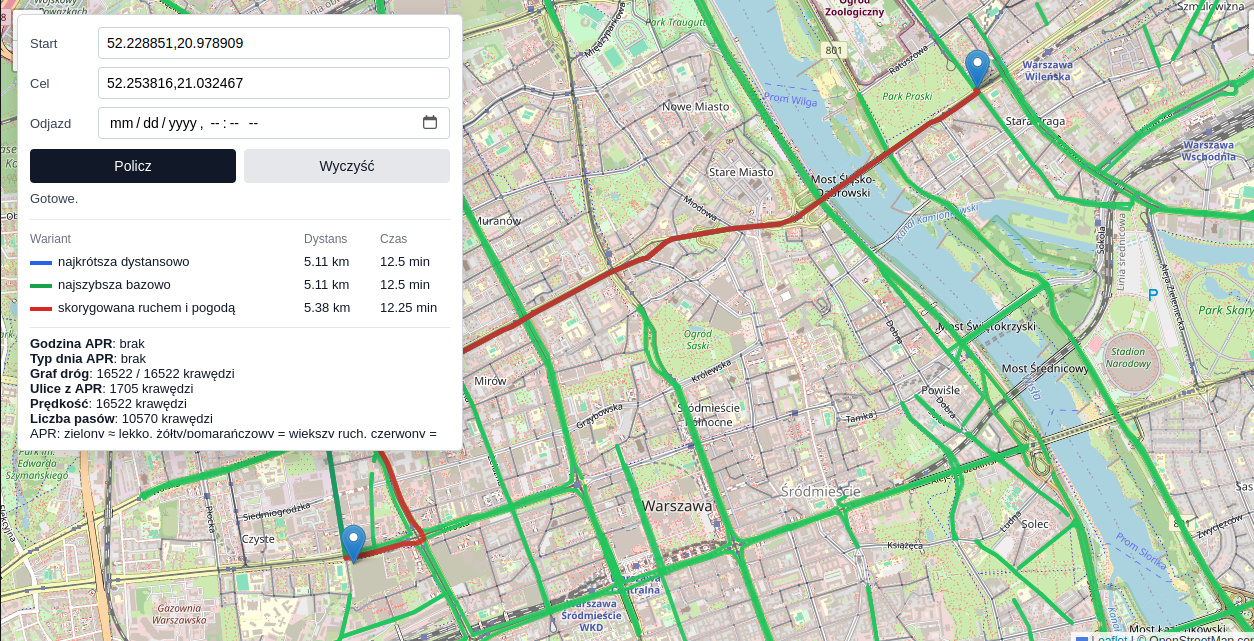
\includegraphics[width=\textwidth]{png/short_variant_opennavigation.png}
        \subcaption{Wyniki aplikacji OpenNavigation}
    \end{subfigure}
    \hfill
    \begin{subfigure}[t]{0.45\textwidth}
        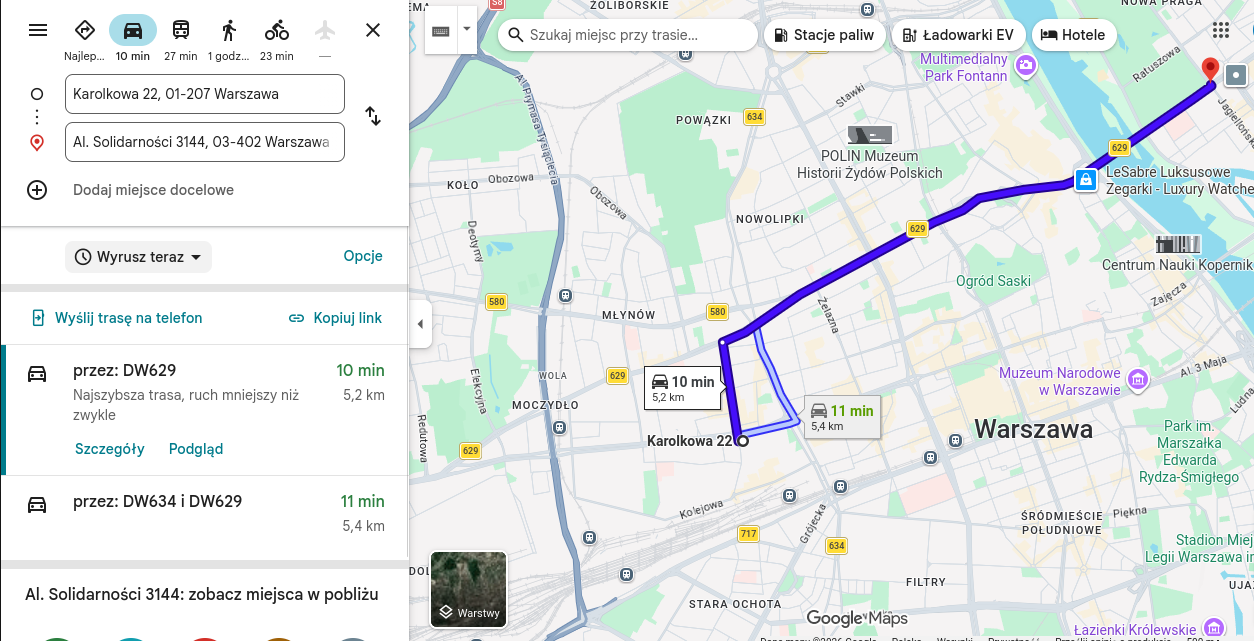
\includegraphics[width=\textwidth]{png/short_variant_google.png}
        \subcaption{Wyniki Google Maps}
    \end{subfigure}
    \caption{Przykład krótkiej trasy}
\end{figure}

\begin{figure}[H]
    \begin{subfigure}[t]{0.45\textwidth}
        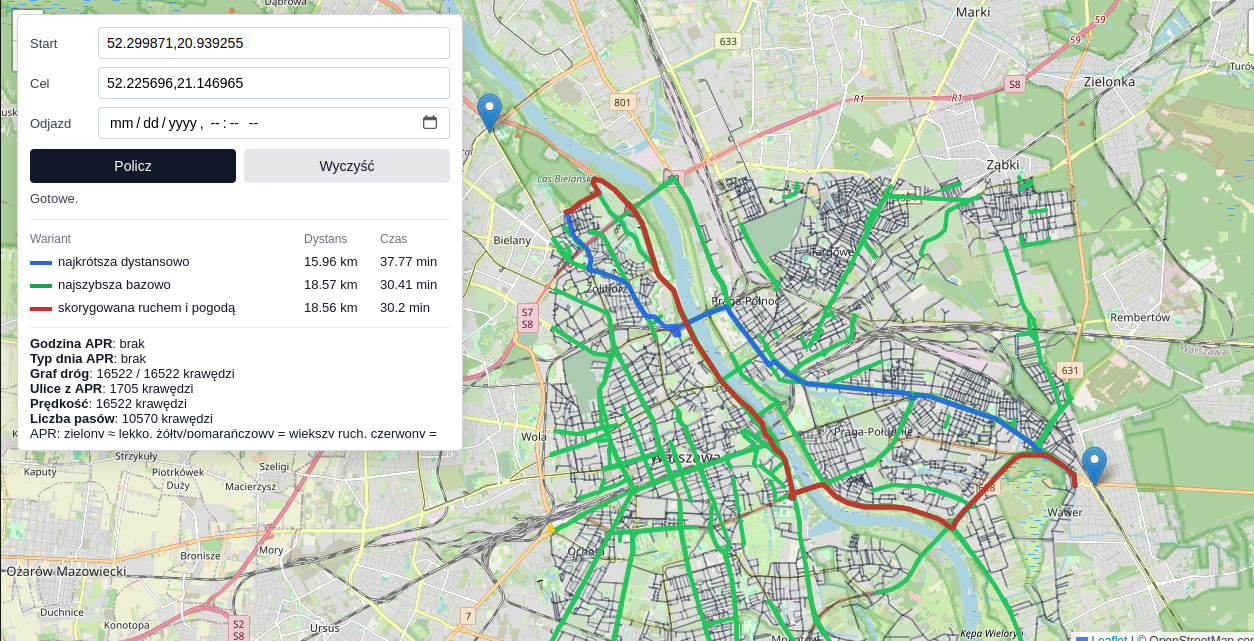
\includegraphics[width=\textwidth]{png/long_variant_opennavigation.png}
        \subcaption{Wyniki aplikacji OpenNavigation}
    \end{subfigure}
    \hfill
    \begin{subfigure}[t]{0.45\textwidth}
        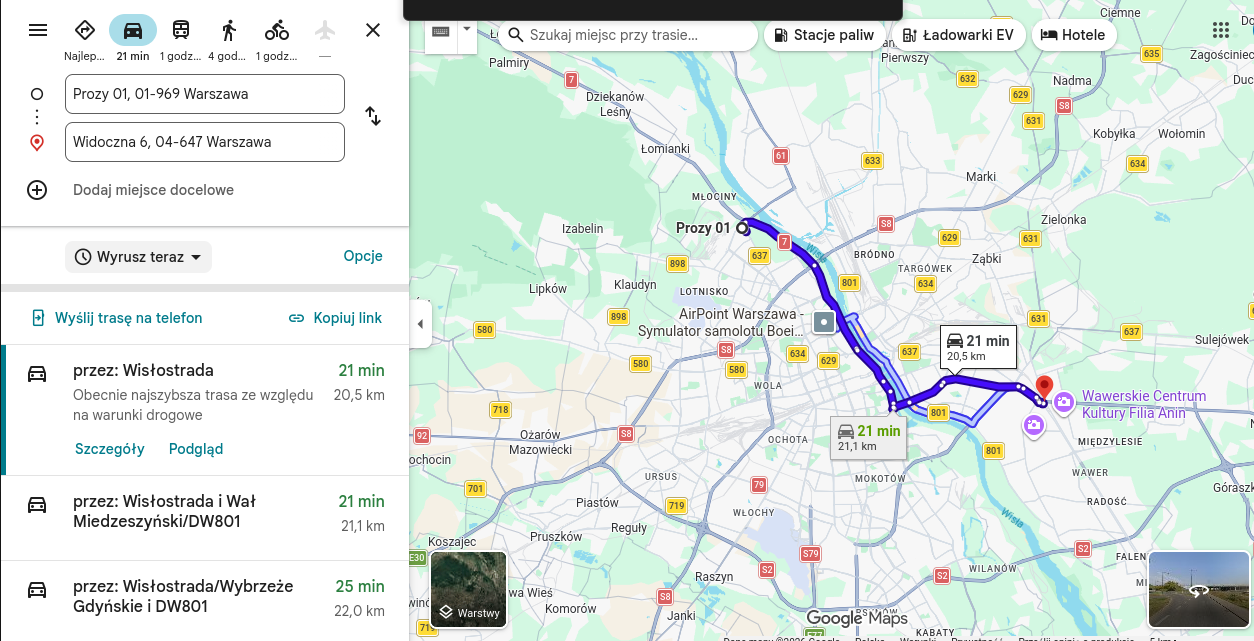
\includegraphics[width=\textwidth]{png/long_variant_google.png}
        \subcaption{Wyniki Google Maps}
    \end{subfigure}
    \caption{Przykład długiej trasy}
\end{figure}

\begin{figure}[H]
    \begin{subfigure}[t]{0.45\textwidth}
        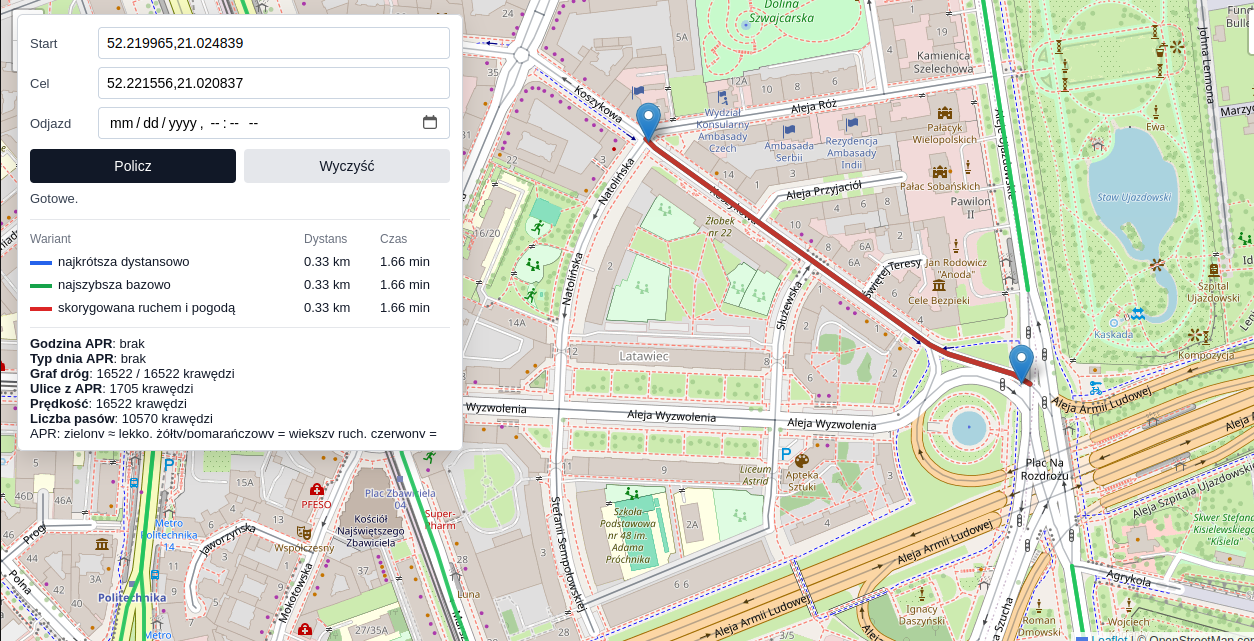
\includegraphics[width=\textwidth]{png/ultra_short_variant_opennavigation.png}
        \subcaption{Wyniki aplikacji OpenNavigation}
    \end{subfigure}
    \hfill
    \begin{subfigure}[t]{0.45\textwidth}
        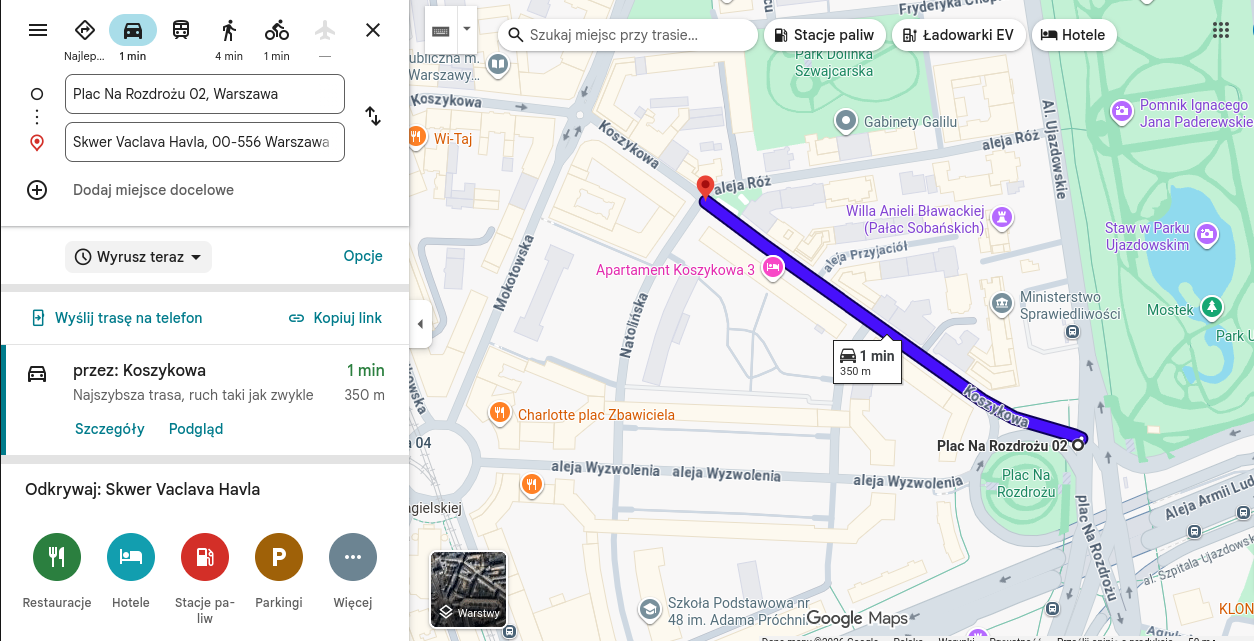
\includegraphics[width=\textwidth]{png/ultra_short_variant_google_maps.png}
        \subcaption{Wyniki Google Maps}
    \end{subfigure}
    \caption{Przykład trasy ultrakrótkiej}
\end{figure}

\begin{figure}[H]
    \begin{subfigure}[t]{0.45\textwidth}
        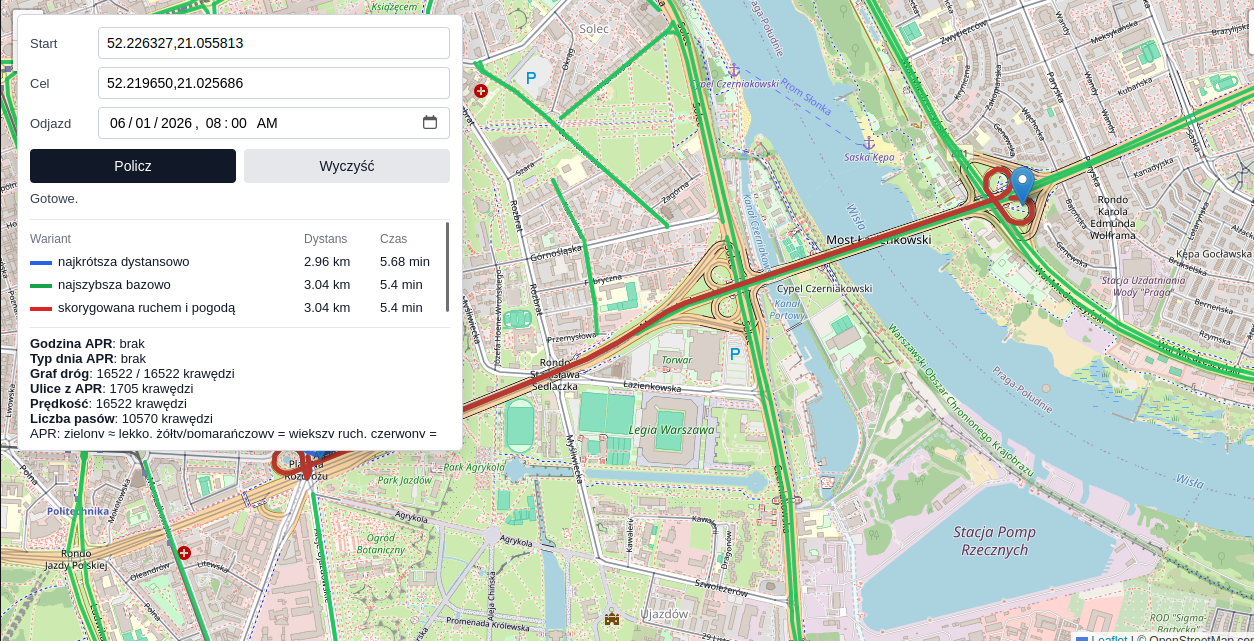
\includegraphics[width=\textwidth]{png/morning_peak.png}
        \subcaption{Wyniki aplikacji OpenNavigation}
    \end{subfigure}
    \hfill
    \begin{subfigure}[t]{0.45\textwidth}
        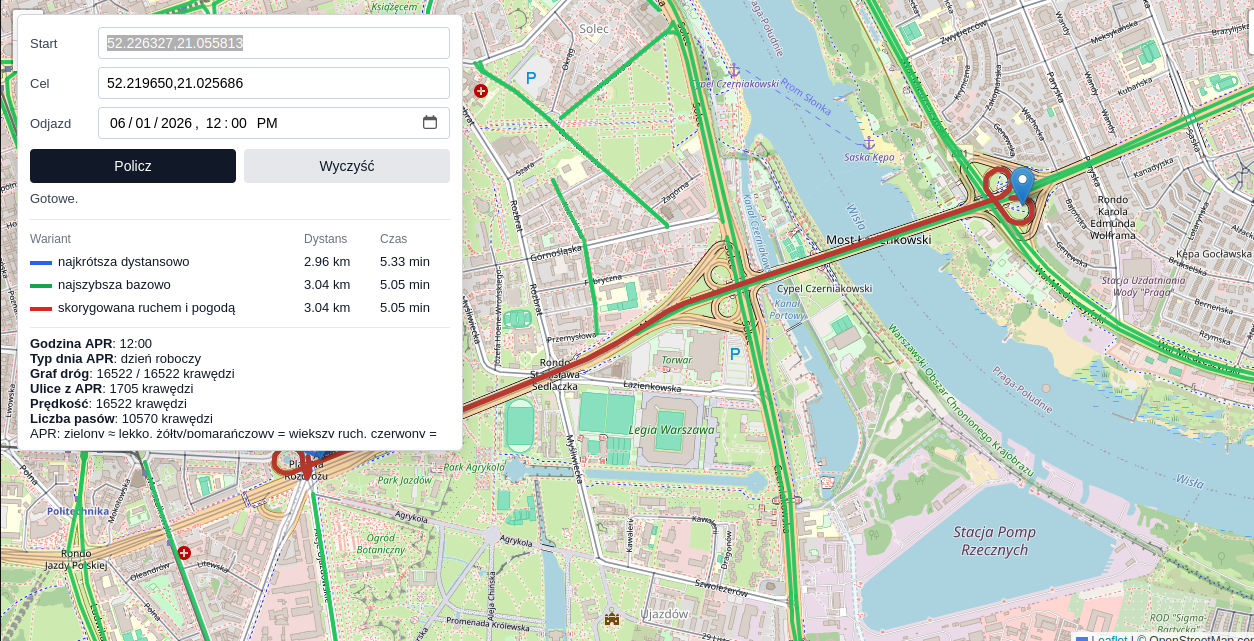
\includegraphics[width=\textwidth]{png/midday.png}
        \subcaption{Wyniki Google Maps}
    \end{subfigure}
    \caption{Porównanie porannych godzin szczytu z ruchem w południe na krótkim odcinku}
\end{figure}

\begin{figure}[H]
    \begin{subfigure}[t]{0.45\textwidth}
        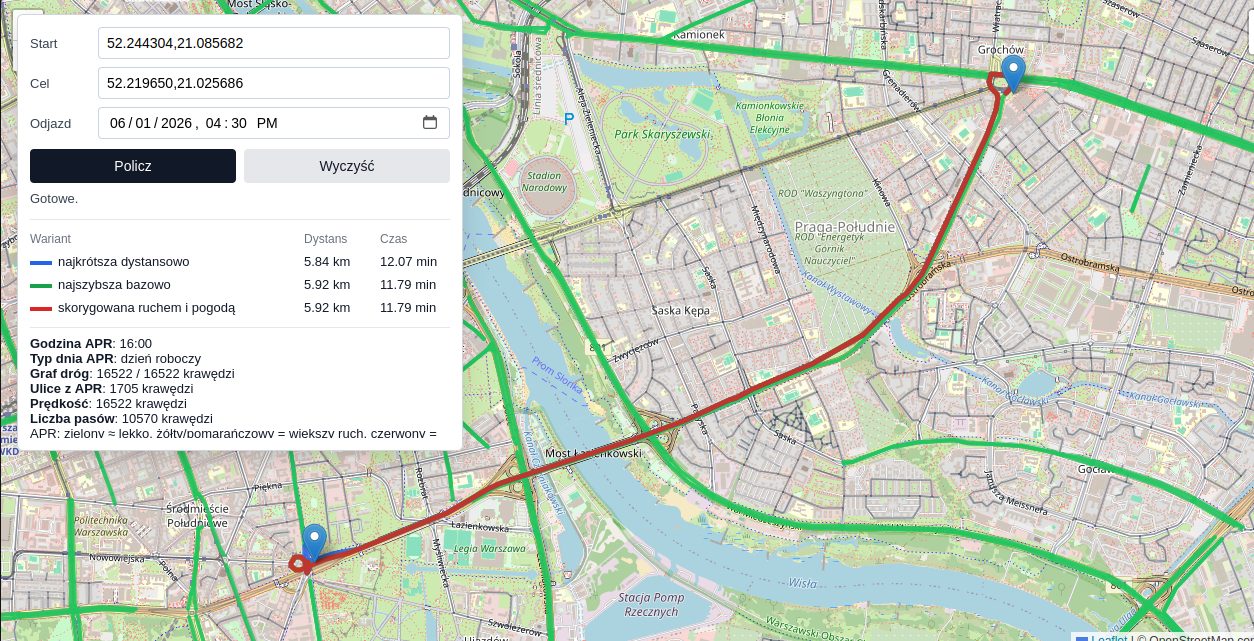
\includegraphics[width=\textwidth]{png/afternoon_peak.png}
        \subcaption{Wyniki aplikacji OpenNavigation}
    \end{subfigure}
    \hfill
    \begin{subfigure}[t]{0.45\textwidth}
        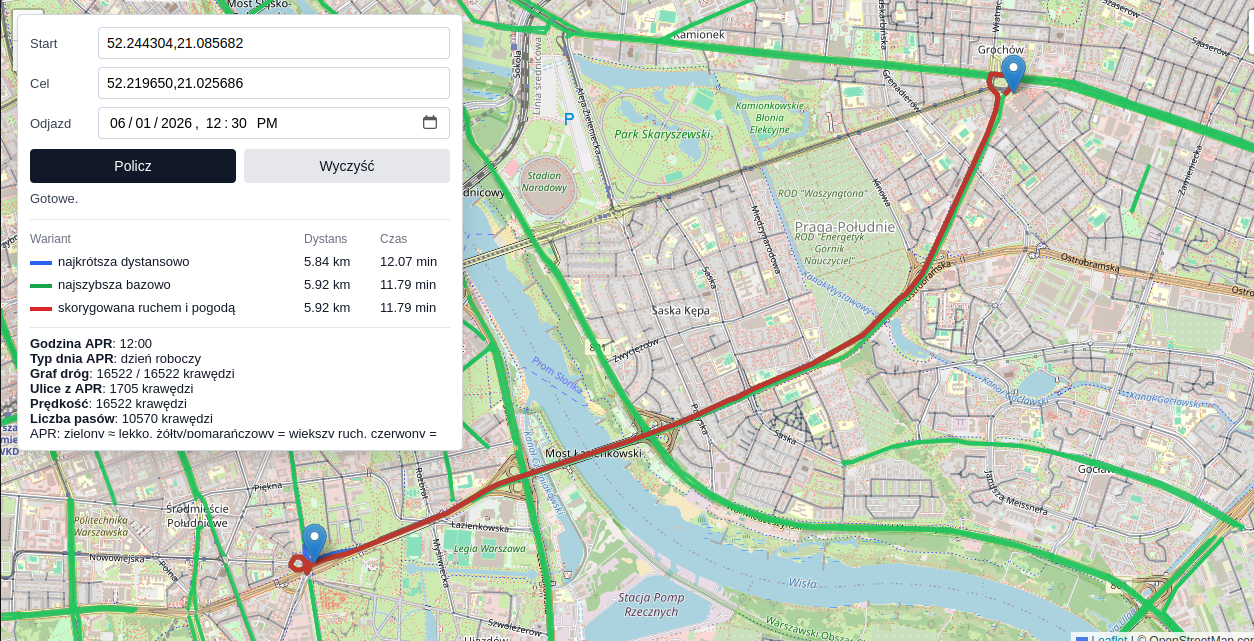
\includegraphics[width=\textwidth]{png/midday2.png}
        \subcaption{Wyniki Google Maps}
    \end{subfigure}
    \caption{Porównanie popołudniowych godzin szczytu z ruchem w południe na dłuższym odcinku}
\end{figure}

\subsection{Wnioski}
Na podstawie porównań można stwierdzić, że algorytm konsekwentnie wyznacza trzy warianty tras
i poprawnie różnicuje je według przyjętych miar (dystans, czas bazowy, czas skorygowany).
Korekta kosztu na podstawie danych ZDM i pogody potrafi zmienić wybór trasy i obniżyć czas
przejazdu względem wariantu bazowego, co potwierdza sens wykorzystania tych źródeł w celu analizy. Różnice względem Google Maps
wskazują na potrzebę dostosowania współczynników oraz uzupełnienia ograniczeń w grafie OSM
(np. zakazy skrętu, zamknięcia). \\
Algorytm skorygowany radzi sobie lepiej niż bazowy oraz najkrótszy, jednak nadal nie obsługuje 
ruchu w czasie rzeczywistym, co oznacza że nie powinien być używany do omijania aktualnych zagęszczeń i korków na trasach, 
a raczej do planowania trasy z uwzględnieniem danych historycznych i kontekstowych. Warto zauważyć, że korekcja trasy
w aplikacji w przypadku tras krótkich była na korzyść w stosunku do danych z Google Maps, natomiast
w przypadku tras długich było odwrotnie.

\section{Dalsze kierunki badania}
W kolejnych etapach powinniśmy skupić się na poprawieniu znajdowania najszybszej trasy oraz
poprawie szacowania czasu przejazdu. W tym celu należy rozważyć następujące kierunki:
\begin{itemize}
    \item \textbf{Kalibracja współczynników} -- zmiana \textit{traffic\_factor} oraz
    \textit{speed\_factor} aby poprawić trafność wyznaczanych tras.
    \item \textbf{Ograniczenia drogowe} -- uzupełnienie grafu OSM o zakazy skrętu,
    zamknięcia i ograniczenia kierunkowe, aby ograniczyć rozbieżności z rzeczywistymi trasami.
    \item \textbf{Dane czasu rzeczywistego} -- dodanie często aktualizowanych źródeł
    (np. zdarzenia drogowe, zagęszczenia ruchu).
    \item \textbf{Walidacja zewnętrzna} -- porównanie wyników z rzeczywistymi czasami przejazdu z łatwo dostępnych źródeł (Google Maps nie daje możliwości łatwego zautomatyzowania tworzenia własnych tras)
\end{itemize}


\section{Podsumowanie}

W raporcie przedstawiono zbudowaną infrastrukturę projektu oraz zarys potoku przetwarzania danych,
który obejmuje pobór danych, buforowanie w Kafka, przetwarzanie w Spark i zapis wyników do
struktury katalogów projektu. Opisano kluczowe źródła danych wraz z formatami i przykładowymi 
wynikami zapytań, co stanowi podstawę do budowy grafu dróg i korekty kosztów przejazdu.

W części analitycznej występuje wstępne porównania wariantów tras dla kilku par punktów,
zestawiając wyniki programu z danymi z Google Maps. Analiza pokazuje, że algorytmy poprawnie
generują warianty tras pod kątem dystansu i czasu, a korekty na podstawie danych ZDM i pogody
potrafią poprawić wynik, choć wciąż występują rozbieżności wynikające z ograniczeń danych
oraz uproszczeń w grafie OSM.

Zidentyfikowane ograniczenia wskazują na potrzebę dalszej kalibracji współczynników i
uzupełnienia ograniczeń drogowych oraz rozbudowy źródeł danych. Zaproponowane kierunki badań
koncentrują się na poprawie trafności wyznaczania tras i zbliżeniu wyników do rzeczywistych
czasów przejazdu.



\end{document}